\section{Rezultati}
Kao što smo već spomenuli, model ispitujemo na skupu slika CelebA, povećavajući rezoluciju od $4 \times 4$ do $64 \times 64$. Primjer promjene rezolucije prikazan je na slici \ref{gt_resolutions}.

\begin{figure}[h]
\centering
		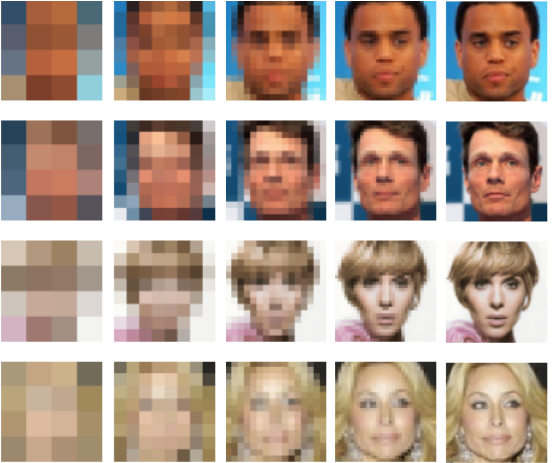
\includegraphics[width=0.7\textwidth]{images/ground_truth/gt_resolutions.png}
\caption{Slike iz skupa CelebA rastuće rezolucije, od $4 \times 4$ do $64 \times 64$.}
\label{gt_resolutions}
\end{figure}

Prilikom generiranja slika za demonstraciju, koristimo se "trikom odsijecanja" \engl{truncation trick}: uzorkujemo iz normalne razdiobe, ali ako prelazi određeni prag, uzorak odbacujemo i ponavljamo postupak. Ideja je da ovim pristupom poboljšavamo kvalitetu generiranih slika, ali gubimo na određenom stupnju raznolikosti. Napomenimo još da se prilikom evaluacije rezultata ovime ipak ne koristimo.

Uzorak slika iz odabranog modela nakon treniranja uz veličinu minigrupe od 16 primjera te podešavanje parametara prikazani su na slici \ref{generated_16bs_fine_tune}.

\begin{figure}[h]
\centering
		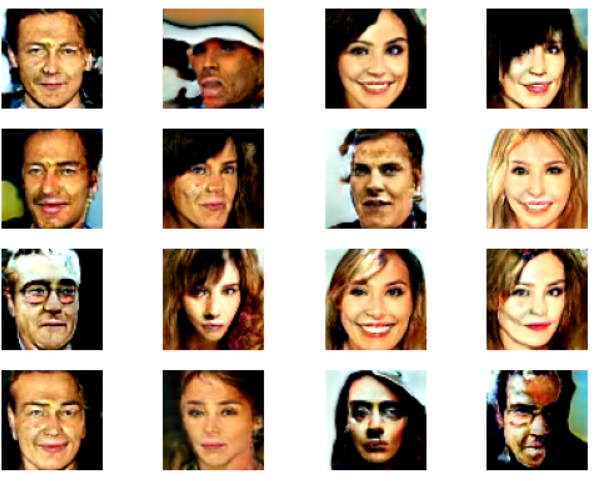
\includegraphics[width=0.8\textwidth]{images/generated/16bs_best_fid.png}
\caption{Uzorak slika generiran odabranim modelom uz minigrupu od 16 primjera}
\label{generated_16bs_fine_tune}
\end{figure}

FID određen na skupu za testiranje (oko 50000 slika) kroz epohe na najvišoj rezoluciji prikazan je u tablici \ref{tablica_fid_16bs}. Iako ne postoji konsenzus pomoću kojeg skupa odrediti FID, prema \todo{are all gans created equal} odlučili smo se za skup za testiranje radi pravednije procjene.

\begin{table}[h]
\caption{FID vrijednosti modela kroz epohe treniranja}
\begin{center}
\begin{tabular}{ |c|c|c|c|c|c|c|c|c|} 
 \hline
 Epoha & 1 & 2 & 3 & 4 & 5 & 6 & 7 & 8 \\
 \hline
 FID & 2221.56 & 2563.519 & 2042.023 & 2973.36 & 2061.18 & 2025.02 & 2222.09 & 1770.68 \\
 \hline
\end{tabular}
\end{center}
\label{tablica_fid_16bs}
\end{table}

Da bismo dodatno podesili parametre, trebali smo odabrati epohu da inicijaliziramo parametre temeljem te vrijednosti. Odabrali smo treću epohu, iako imamo i slučajeve gdje je FID vrijednost niža. Ovo se temelji na pregledavanju slika koje je model generirao u pojedinom stadiju. Primjer generiranih slika u zadnjoj epohi treniranja prikazan je na slici \ref{generated_lowest_fid}.

\begin{figure}[h]
\centering
		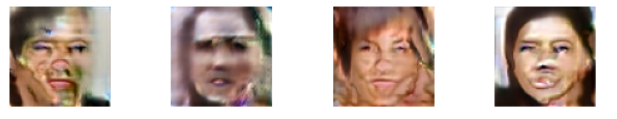
\includegraphics[width=0.8\textwidth]{images/generated/16bs_lowest_fid.png}
\caption{Uzorak slika generiran modelom s najmanjim FID-om}
\label{generated_lowest_fid}
\end{figure}

Osim ovog pristupa, pokušan je i pristup gdje povećamo veličinu grupe na 64 primjera, a težine modela nižih rezolucija s najboljim FID-om koristimo kao osnovu za više rezolucije. Međutim, nisu dobivena značajna vizualna poboljšanja. 

U kasnijim epohama treniranja, vrlo lako se mogla primijetiti pojava \textit{mode collapse}. Slika \ref{mode_collapse} pokazuje kako to točno izgleda. 

\begin{figure}[h]
\centering
		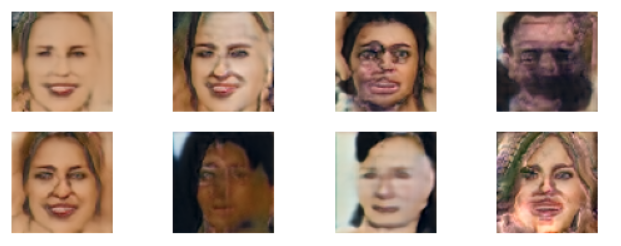
\includegraphics[width=0.8\textwidth]{images/generated/mode_collapse.png}
\caption{Primjer pojave \textit{mode collapse}}
\label{mode_collapse}
\end{figure}

Jedno zanimljivo svojstvo koje posjeduju generativne suparničke mreže jest da se aritmetika nad latentnim vektorima $\vec{z}$ na neki način preslikava u semantiku na generiranim slikama. Slika \ref{interpolation} prikazuje slike generirane latentnim vektorima dobivenim interpolacijom između dva početna latentna vektora. 

\begin{figure}[h]
\centering
		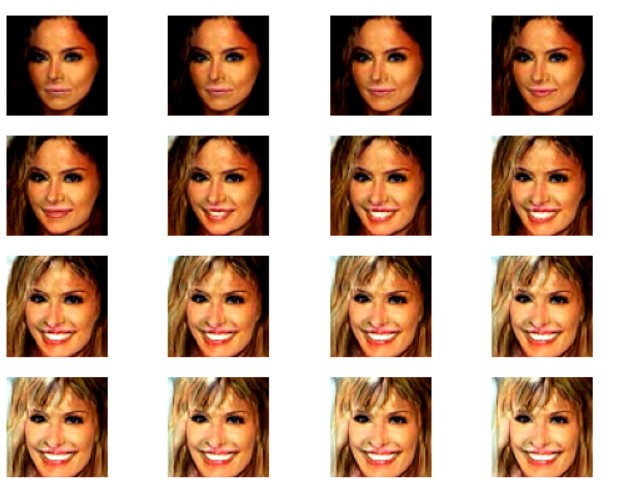
\includegraphics[width=0.8\textwidth]{images/generated/interpolation_1.png}
\caption{Slike dobivene interpolacijom}
\label{interpolation}
\end{figure}

Možemo primijetiti da se između početne i završne slike događa postupna promjena u izrazu lica, boji kose i tenu. To upućuje na zaključak da je model ulazni vektor uspio upotrijebiti kao uputu za generiranje semantičkih elemenata lica, iako raspolaže samo s pojedinim pikselima - u stanju je steći znanje o strukturi lica. Ovu pojavu nazivamo raspetljanošću \engl{disentaglement} latentnog prostora i opisuje sposobnost modela da različita povezana područja ulaznog prostora namijeni za generiranje pojedinih elemenata slike, ali tako da su ta područja specijalizirana. Iako trenutno imamo vrlo malo kontrole nad izlazom modela, raspetljanost ulaznog prostora mogla bi se u budućnosti iskoristiti da riješimo i taj izazov.